\subsubsection{ Nguyên lý hoạt động}
Tác vụ "Temperature and Humidity Monitoring" đóng vai trò là khối thu thập dữ liệu trung tâm (Producer) của toàn bộ hệ thống. Tác vụ này có trách nhiệm giao tiếp với cảm biến DHT20 qua chuẩn I2C để trích xuất nhiệt độ và độ ẩm, hiển thị trực quan lên màn hình LCD 16x2, đồng thời cung cấp dữ liệu đầu vào cho các tác vụ phân tích và cảnh báo khác.

Nguyên lý hoạt động được chia thành các bước kiểm duyệt và xử lý chặt chẽ:
\begin{itemize}
    \item \textbf{Kiểm duyệt dữ liệu (Data Validation):} Sau mỗi lần đọc cảm biến, hệ thống sử dụng hàm \texttt{isnan()} để kiểm tra tính hợp lệ của dữ liệu. Nếu xuất hiện lỗi đọc (NaN), hệ thống sẽ in cảnh báo ra Serial, tạm dừng 1000ms và lặp lại quá trình đọc mà không làm thay đổi trạng thái của các biến toàn cục. Điều này giúp bảo vệ hệ thống khỏi các giá trị nhiễu hoặc rác.
    \item \textbf{Hiển thị có điều kiện (Conditional Display):} Dữ liệu hợp lệ sẽ được so sánh với ngưỡng nhiệt độ \texttt{glob\_temp\_threshold} (có thể được cập nhật động từ nền tảng CoreIoT).
    \begin{itemize}
        \item \textbf{Môi trường bình thường ($T \le$ Threshold):} LCD hiển thị trực quan Độ ẩm (H) ở hàng trên và Nhiệt độ (T) ở hàng dưới. Hệ thống duy trì trạng thái này trong chu kỳ 1000ms trước khi cập nhật mẫu mới.
        \item \textbf{Vượt ngưỡng cảnh báo ($T >$ Threshold):} LCD ngay lập tức chuyển sang chế độ báo động. Hàng dưới chốt cứng thông số nhiệt độ hiện tại kèm mức ngưỡng vi phạm. Hàng trên thực hiện hiệu ứng chớp tắt dòng chữ "\texttt{! WARNING TEMP !}" 5 lần (chu kỳ 500ms sáng / 500ms tắt, tổng thời gian 5000ms) để thu hút tối đa sự chú ý của người dùng mà không làm gián đoạn hệ điều hành (nhờ \texttt{vTaskDelay}).
    \end{itemize}
\end{itemize}

\subsubsection{Cơ chế điều phối hệ thống bằng Semaphore}
Khác với Task 1 và Task 2 đóng vai trò là "Consumer", Task giám sát nhiệt ẩm hoạt động như một "Producer". Ngay khi dữ liệu hợp lệ được ghi vào biến toàn cục \texttt{glob\_temperature} và \texttt{glob\_humidity}, tác vụ này lập tức phát tín hiệu đánh thức các phân hệ khác bằng cách giải phóng đồng thời 3 Binary Semaphore:
\begin{enumerate}
    \item \texttt{xBinarySemaphoreTemp\_blinky}: Kích hoạt tính toán lại tần số nháy LED1.
    \item \texttt{xBinarySemaphoreTemp\_neo}: Kích hoạt đánh giá màu sắc dải LED NeoPixel.
    \item \texttt{xBinarySemaphoreTinyMLData}: Kích hoạt bộ nội suy Machine Learning (Naive Bayes) để dự đoán nhãn trạng thái môi trường.
\end{enumerate}


\subsubsection{Sơ đồ máy trạng thái (FSM)}



\begin{figure}[H]
\centering
    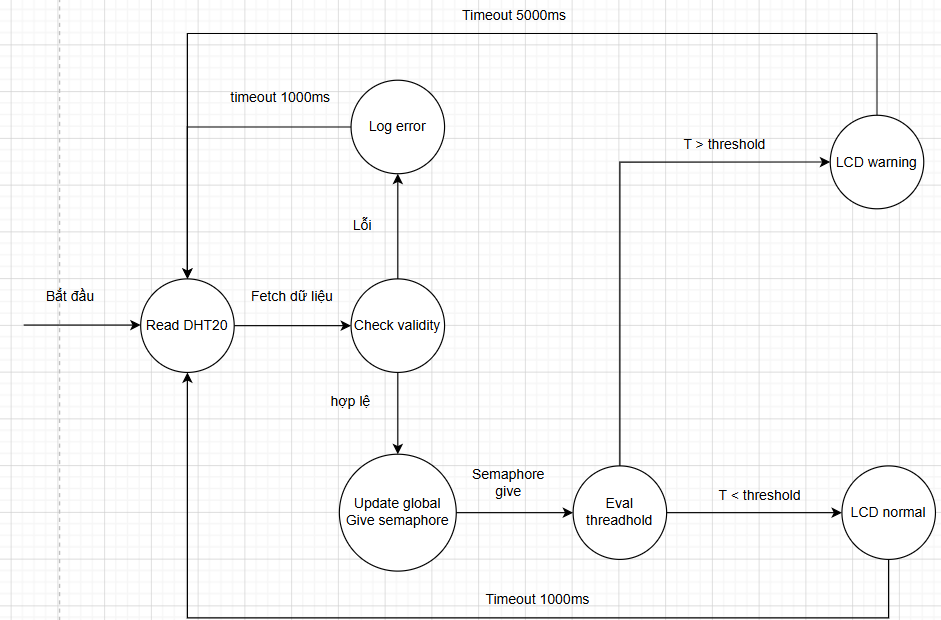
\includegraphics[width=1\linewidth]{picture/task_3_fsm.png}
 \caption{Task 3 FSM}
\end{figure}
